\chapter[Data selection and vacuum arcs localisation]{Data selection and vacuum arcs localisation}

\section[Offline selection of the events]{Offline selection of the events}

In order to perform the data analysis, a full analysis framework have been developed using MATLAB. The selection of the interesting events will be described chronologically, as it's performed in the analysis program.

\subsection[Data collected from the PXI]{Data collected from the PXI}

As mentioned in the previous chapter, the data acquisition is performed from a real-time LabVIEW program running in the PXI crate. When an event hits at least one of the online triggers is saved into the crate's disk. Every 8 hours, the crate assemble a data file and stores it in TDMS format~\cite{NI:TDMS}. 

In order to proceed with the analysis, the files are merged joining all the data of the same day together in a new data file. The original data are anyway kept stored.

The kind of events that are collected by the PXI crate have two natures, and are flagged differently depending wether they belong to:
\begin{enumerate}
\item Interlock pulses: an event that triggered at least one of the online interlock. If available, the two precedent pulses are saved.
\item Backup pulses: the data of a pulse are saved once per minute.
\end{enumerate}
The first ones are sent to the next analysis step, the second ones are analysed separately to check the running condition of the accelerator and the RF systems.


\newpage
\subsection[Power spikes detection]{Power spikes detection}

A key operational issue is the presence of power spikes, that sometimes are detected in the systems. The main characteristics of these events are:
\begin{itemize}
\item Short duration: normally in the range 10-100 ns
\item Very high power burst: it can reach 60-70 MW or even more 
\end{itemize}
The fist point makes the spikes easily detectable using a frequency filter to detect signals of that short duration. 

 After careful investigation, the origin of the spikes has been addressed to the TWT. It has to be pointed out that the frequency of the spikes is anyway low compared to the rate of the breakdown, and that after the first runs the replacement of a very active tube improved a lot the performance. As can be seen in Fig. \ref{spikesAndDetuning}, the spike can happen everywhere in the pulse.

 \begin{figure}[h]
 \centering
   \subfigure[Power spike in the prepulse]
   {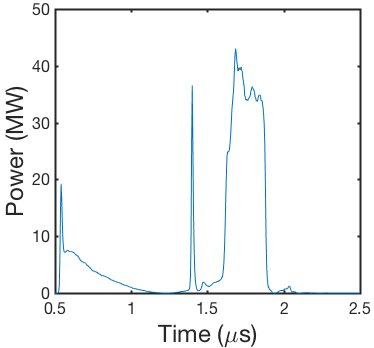
\includegraphics[scale=0.48]{pictures/spike1.png}}
 \hspace{2mm}
 \subfigure[Power spike in the compressed pulse]
   {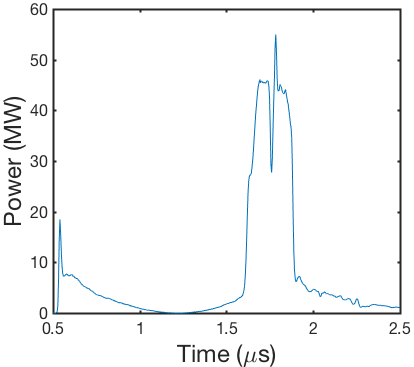
\includegraphics[scale=0.46]{pictures/spike2.png}}
 \caption{Cavity input power signal for two different spikes. Spikes can happen anywhere in the signal, even if the experience suggest that are more likely in the compressed pulse.}
 \label{spikesAndDetuning}
 \end{figure}


When a spike gets detected, the correspondent interlock is sorted out, and also the followings for a given period of time (generally 90 s). The reason is that it is believed that the burst of power brought from the spike may trigger strong breakdowns that damage the surface. This creates new emitters that triggers new breakdowns as soon as the system don't reach an equilibrium. The waiting time before restarting to count the breakdowns gives time to the surface to cool down and get reconditioned.


\subsection[Pulse compressor tuning issues]{Pulse compressor tuning issues}
\label{sec:PCtune}

RF tests of accelerating cavities are carried out using the CLIC nominal pulse shown in Fig. \ref{detuning_fig} (a). This comes from the necessity to find a common test protocol for accelerating cavities, that has also to match the different pulse length of the RF foreseen in the three stages of the CLIC implementation. To meet these requirements, the CLIC nominal pulse is made of a filling (or rising) time of 70 ns and a flat-top 180 ns long.

A common operational issue is the detuning of the pulse compressor, that provokes an imperfect shape of the RF pulse. This event does not constitute an issue for the implementation of CLIC (unless implemented in the klystron option). Anyway excessively detuned running periods are sorted out, hence far from the wanted experimental conditions. 

 \begin{figure}[h]
 \centering
  \subfigure[CLIC nominal pulse]
   {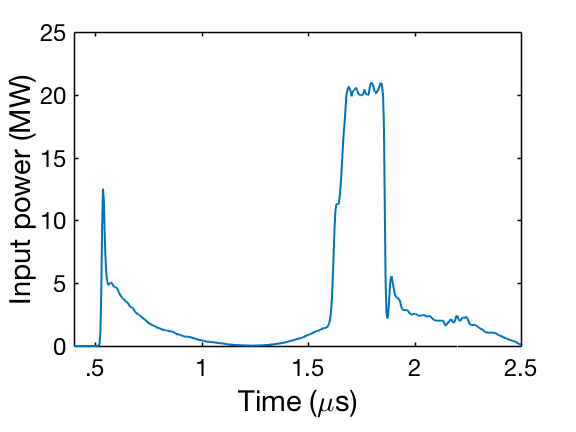
\includegraphics[scale=0.45]{pictures/CLIC_nominal_pulse.png}}
  \subfigure[Pulse compressor undertuned]
   {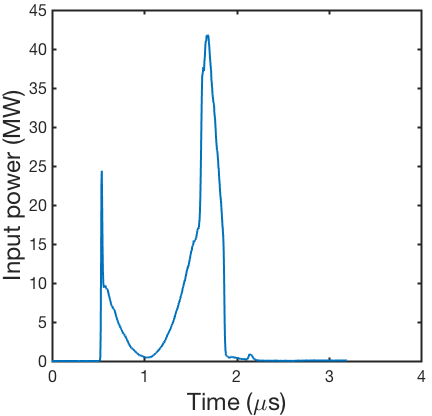
\includegraphics[scale=0.42]{pictures/Undertuning.png}}
 \hspace{2mm}
 \subfigure[Pulse compressor overtuned]
   {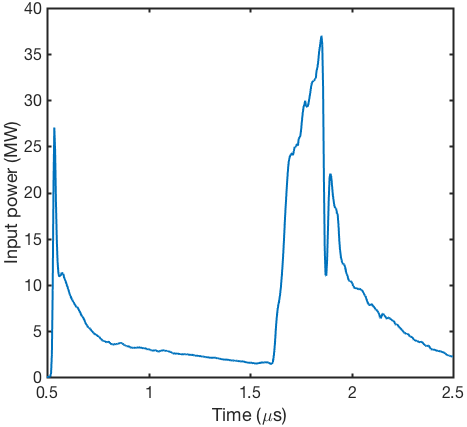
\includegraphics[scale=0.41]{pictures/Overtuning.png}}
\caption{The CLIC nominal pulse and two extreme cases of detuning of the pulse compressor.}
 \label{detuning_fig}
 \end{figure}


The origin of the detuning is the difference of the total volume of the pulse compressor's cavities. This is controlled changing the cooling water temperature, but as any other thermal system needs time for the regulation \cite{Woolley:CWS2016}. The detuning is a particular issue in summer, when the thermal excursion during the day is particularly high.

As general rule a slight detuning of the pulse is tolerated, and it is not possible to get rid of it because the regulation of the temperature of the chillers act dynamically and needs time to compensate the variations. On the other hand the data are discarded in case of extreme detuning such as in Fig. \ref{detuning_fig} (b) and (c), where the box-shape of the pulse is not recognisable anymore.



\subsection[The metric]{The metric}

The online selection of the events is not strict enough to select immediately just the breakdowns happening in the structure. This is made on purpose in order to not to risk to lose any interesting event, but makes an additional filtering level necessary. 
In order to sort out the non-interesting or fake breakdowns two quantities are calculated:
\begin{equation}
m_{\text{REF}}  =  \frac{ U_{INC} -  U_{REF}   }{  U_{INC} + U_{REF}   }
\end{equation}
\begin{equation}
m_{\text{TRA}}  =  \frac{ U_{INC} -  U_{TRA}   }{  U_{INC} +  U_{TRA}   }
\end{equation}
where has been evaluated the signal energy U from the power signal over the whole acquisition period T
\begin{equation}
U = \int_0^T P(t) \, dt
\end{equation}
For a non-breakdown event it will be $m_{\text{REF}} \sim 1$ and $m_{\text{TRA}} \sim 0$.

Plotting this two classifiers, two distinct regions gets highlighted (see Fig. \ref{Metric_plot}). The upper left region is made of the fake interlocks and the breakdown that happen upstream the structure under test. The events happening in the structure end up in the lower right area on the plot. 

In this work the selection of the events has been performed using the two thresholds plotted in Fig. \ref{Metric_plot}, but as future perspective more refined methods can be used, such as k-means clustering or neural networks \cite{ML:book}.

\begin{figure}[h]
\centering 
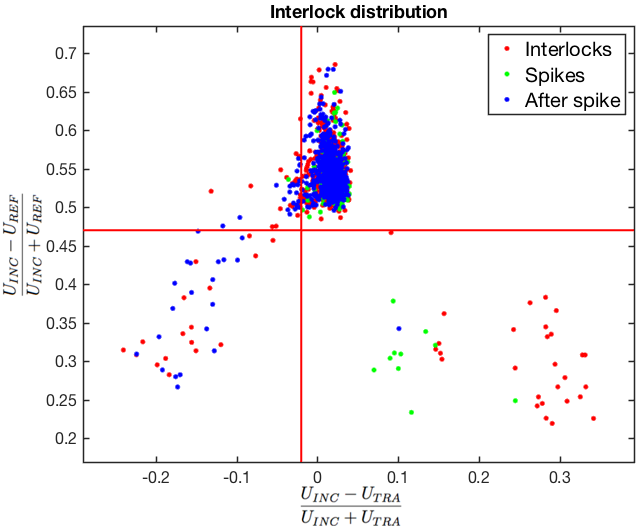
\includegraphics[scale=0.6]{pictures/metric_plt.png}
\caption{Metric plot for an unloaded run. Data grouped in two different regions are clearly visible. The lowest region is containing the interesting interlocks, that are sent to the next analysis step}
\label{Metric_plot}
\end{figure}


\subsection{Power back-off failure}
\label{sec:pbof}

According to the test procedure, after a breakdown the input power gets cut for a period of time that is between the 5 and 10 seconds. Afterwards the power is restarted and gets ramped up gradually up to the nominal value unless a new breakdown happens.

The reason of this behaviour is to preserve the surfaces of the accelerating cavity under test. In foreseen of the CLIC operation simulation, the structures will be tested without any buffer period after the breakdown and restoring the input RF at full power. Anyway for the moment no test of that kind has been done, and will be implemented in the future in one of the other test stand at CERN~\cite{Walter:PC}.

For unknown reasons the power is not always cut immediately. This could provoke a breakdown that follows immediately the former one, but that is provoked by the malfunction of the instrumentation that does not cut the power fast enough. For this reason, all the events in the next three seconds after a breakdown are discarded. This is a common procedure carried out also in the other XBOX at CERN, and constitutes an issue that will be investigated in the future. 


\subsection[Additional criteria for runs with beam]{Additional criteria for runs with beam}

During the experiments with beam, two additional conditions have to be met to consider an interlock as a breakdown in the accelerating structure
\begin{enumerate}
\item The beam has to be present during the pulse
\item In the case of a group of successive breakdowns, also called \textit{cluster}, the initial trigger breakdown has to be triggered during a pulse with beam
\end{enumerate}





\section[Time and space positioning of the breakdowns]{Time and space positioning of the breakdowns}

The position detection of the breakdown is based on the RF signals. The RF diagnostic is based on the signals recorded from directional couplers of the incident power (INC), transmitted power (TRA) and reflected power (REF). 

Hence the accelerating structure is well matched with the rest of the RF system, the reflections are minimal. This means that during the normal operation only the INC and TRA are non-zero signals.

When a breakdown happens, the plasma into the structure acts as a short circuit \cite{Degiovanni:2025952}, as effect the RF incoming after the breakdown gets reflected back, and consequently the transmitted power falls. This process is summarised in Fig.~\ref{BD_scheme}. A full dissertation on various possible positioning methods is available in \cite{Rajamaki:2143815}.

\begin{figure}[h]
\centering 
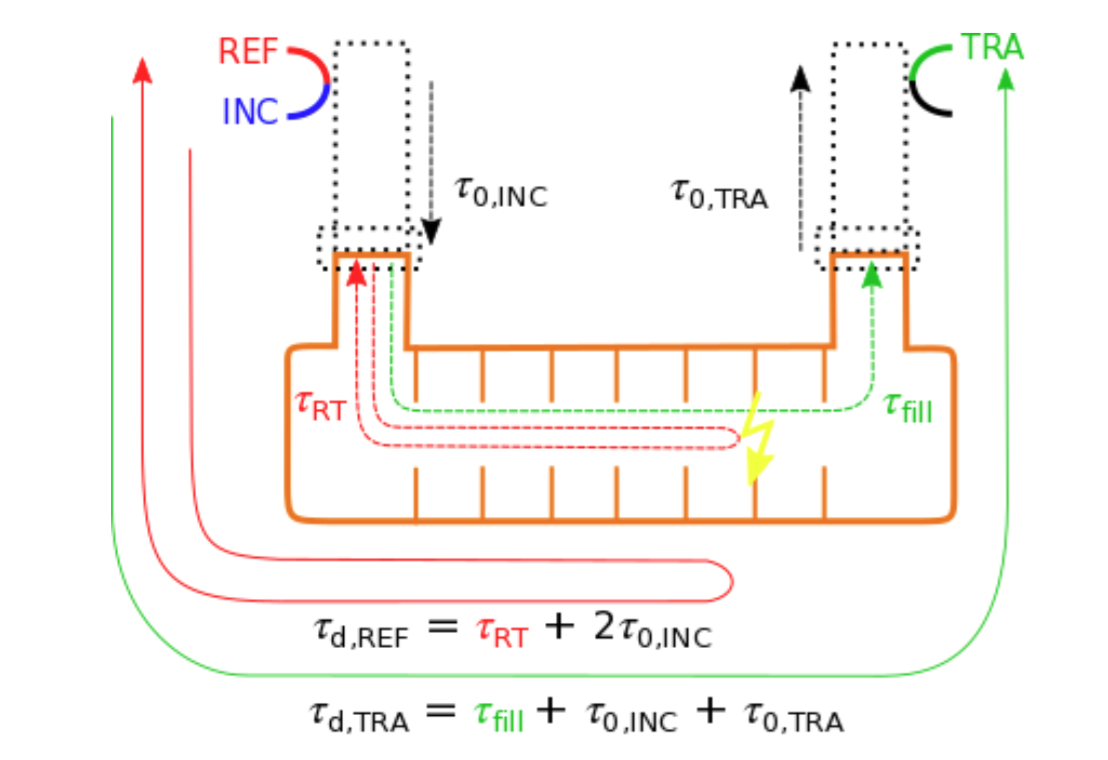
\includegraphics[scale=0.3]{pictures/structure_scheme}
\caption{RF signal time delays in a travelling-wave accelerating structure. In the case under exam, $\tau_{0,\text{INC}}$ = $\tau_{0,\text{TRA}}$}
\label{BD_scheme}
\end{figure}


\subsection[Edge method]{Edge method}

The Edge Method is based on the time difference of arrival of the falling edge of the TRA signal and the rising edge of the REF signal. This method constitutes the most reliable method that is used for breakdown positioning. 

Assuming that the vacuum arc starts to absorb and reflects the RF immediately after being triggered, this method will individuate the longitudinal position of the onset breakdown in the accelerating cavity.

The edges of the TRA and REF signals are individuated looking for the deviation point of the signal from the nominal pulse (see Fig. \ref{dev_pt} (a) ). This is easily done using the previous pulse, which is recorded in the data when a breakdown happens.  According to this method the time delay $\tau_d^{\text{edge}}$ is
\begin{equation}
\tau_d^{\text{edge}} = \tau_{\text{REF}} - (\tau_{\text{TRA}} - \tau_{\text{FILL}})
\end{equation}
where $\tau_{\text{REF}} $ and $\tau_{\text{TRA}}$ are the time position in the signal of the deviation point from the previous pulse of the transmitted and reflected signals, and $\tau_{\text{FILL}}$ is the filling time of the accelerating structure, that is the time necessary for an RF signal to propagate through the structure. This leads to a time delay that is included between zero and $2 \tau_{\text{FILL}}$.

For noisy signals, using the deviation point detection instead of detecting the edge of the signal at a certain height showed an improvement in the performance of the algorithm. It could anyway happens that for some reason the previous pulse was not recorded, in that case the location of the signals edge is entered manually.

 \begin{figure}
\centering
  \subfigure[RF signals of a breakdown event. The deviation points of the signals are highlighted. The dashed lines are the reference signals, given by the previous pulse.]
   {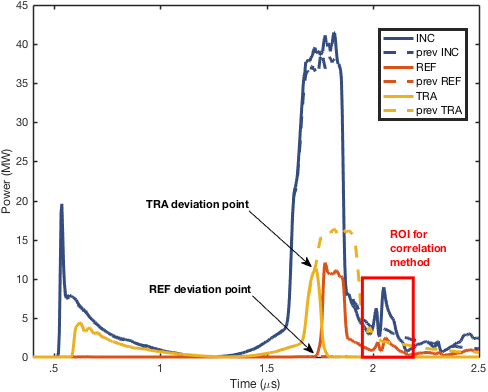
\includegraphics[scale=0.39]{pictures/dev_point.png}}
   \hspace{1mm}
  \subfigure[Detail of the region of interest (ROI) for the correlation method. The dashed lines indicate the time delay between the feature of the signal in exam.]
   {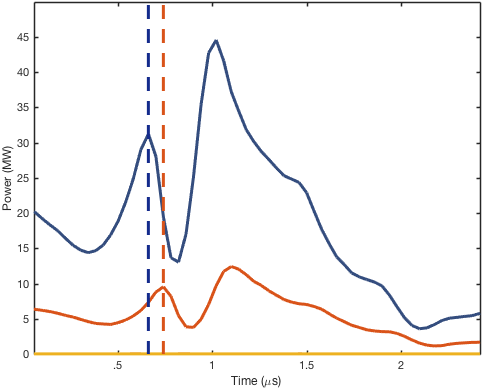
\includegraphics[scale=0.39]{pictures/dev_point_detail_2.png}}
\caption{RF signals of a breakdown in the structure. The plot (b) is the zoom of the region of interest surrounded in red in (a)}
 \label{dev_pt}
 \end{figure}


\subsection[Correlation method]{Correlation method}

It has been outlined before that after the establishment of the breakdown, the INC is reflected back. This means that looking at the tail of the signal after the compressed pulse it is possible to individuate some particular pattern (see Fig. \ref{dev_pt} (b) ), and in a number of cases the same pattern will be visible in the REF signal returning back. 

This method is not always successful since is strongly dependent from two factors: the amplitude of the pattern observed (in Fig. \ref{dev_pt} (b) one of the best example is reported, but most of the times the amplitude is much lower); and the position of the breakdown in the cavity, since the longer is the path of the signal in the structure, the higher will be the attenuation. In order to limit as much as possible the attenuation effect, this analysis is performed using the non-calibrated signals from the log detectors, but it's still not always possible individuate a common pattern between the tails of INC and REF.


\subsection[Comparison of the two methods]{Comparison of the two methods}

It has to be pointed out that the correlation method is not always successful because of the attenuation of the REF signal. In addition, comparing the results of the two methods, the distribution of the arcs in the cavity are definitely different. Figure \ref{edge_vs_corr} shows the difference between the breakdown distribution of the same dataset using the edge (right) and correlation method (left). 

 \begin{figure}[h]
\centering
  \subfigure[Edge method result]
   {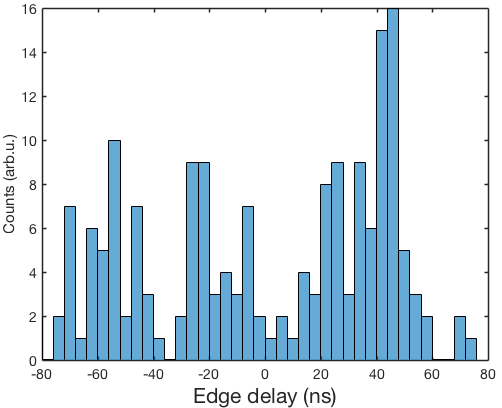
\includegraphics[scale=0.37]{pictures/Exp_UnLoaded43MW_6_edge_method.png}}
   \hspace{1mm}
  \subfigure[Correlation method result]
   {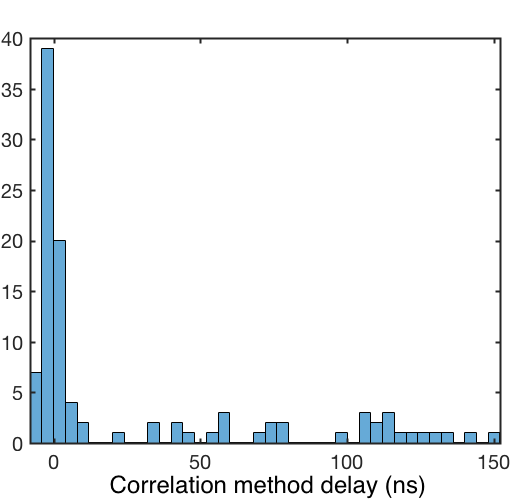
\includegraphics[scale=0.385]{pictures/Exp_UnLoaded43MW_6_correlation_method.png}}
\caption{Comparison of the signals delay distribution for the edge and correlation method in an unloaded run. The spike in proximity of the zero in the correlation delay is visible in any dataset.}
 \label{edge_vs_corr}
 \end{figure}

The distribution obtained using the correlation method present a peak at the beginning of the structure, that is not obtained using the edge method. This overpopulation of breakdowns at the beginning of the structure has been observed in all the dataset processed for this work, but also in \cite{Rajamaki:2143815}.  

Figure \ref{comp_corr_edge} shows the comparison between the two different techniques. The solid line indicate the agreement of the two methods. It is clearly observable that the correlation method is more likely to yield estimates further upstream in the structure than the edge method, as outlined from the asymmetrical distribution. 

An explanation for the asymmetry is given by the \textit{breakdown migration} \cite{Woolley:2015,Jacewicz:CLICWS16,Degiovanni:migration}. According to this hypothesis, if the onset breakdown position is find by the edge method and the position of the steady state stable breakdown is find by the correlation method, then the Fig. \ref{comp_corr_edge} is consistent with the migration upstream in the structure. Downstream migration is not likely, as little or no power is remaining downstream after the arc starts to reflect the incident power. Furthermore, the incident and reflected power can enter in resonance, enhancing even more the field upstream.
A possible migration scenario is presented in Fig. \ref{mig_sc}.

\begin{figure}[h]
\centering 
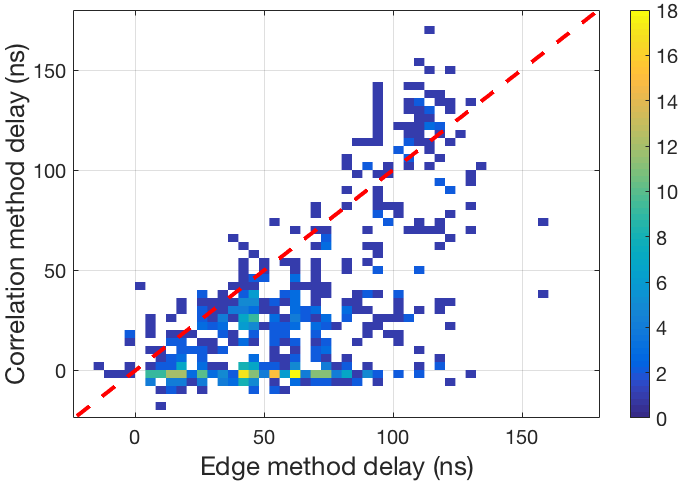
\includegraphics[scale=0.4]{pictures/methods_comparison.png}
\caption{Comparison of edge and correlation method. The straight line represent the accordance of the two methods.}
\label{comp_corr_edge}
\end{figure}

\begin{figure}[h]
\centering 
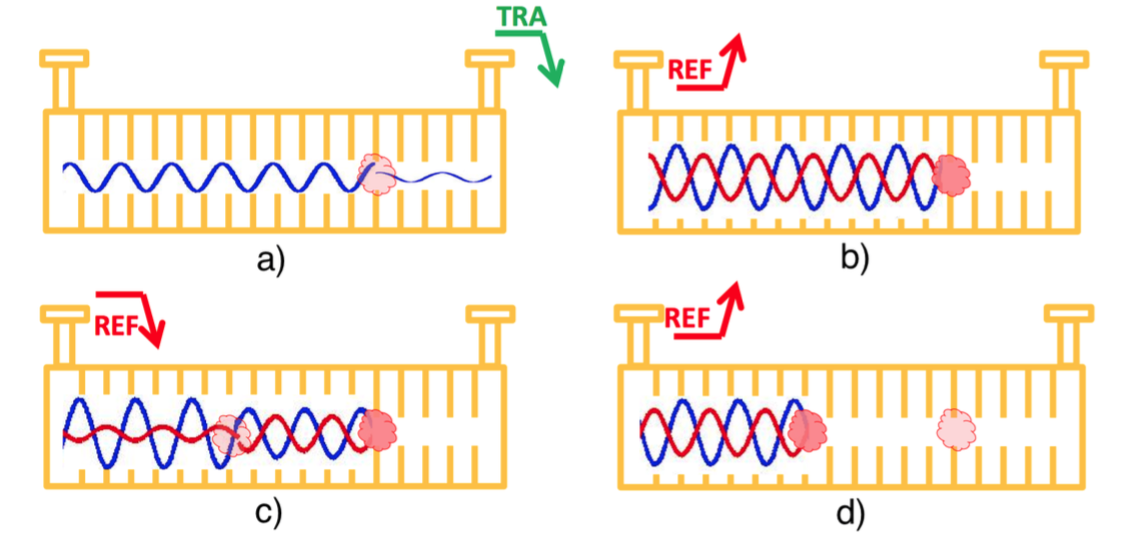
\includegraphics[scale=0.3]{pictures/migration_scenario}
\caption{A possible migration scenario \cite{Degiovanni:migration}: a) A breakdown establish in the structure, absorbing the incident RF; b) The established arc reflects the incident RF; c) Constructive interference between reflected and incident RF provokes another arc upstream; d) As the second arc establish, any remaining power downstream is drained and the first arc gets extinguished}
\label{mig_sc}
\end{figure}




The results of this work are in accord with this theory and constitute an additional proof. Figure \ref{comp_corr_edge} shows that the majority of the breakdown in the loaded condition (in red) are happening in the first part of the structure. The difference is that according to the edge method they are happening in the first half, while the correlation method would place almost all of them at the very beginning. 
This is not surprising, because after the breakdown just the upstream part of the structure remains powered as in the unloaded case, but in addition, the field is much higher in the upstream cells because of the loading. This second effect might act on the migration length of the breakdown, enhancing it. 

To verify this last affirmation, the experiment should be repeated scanning the beam current.

Considering the problems highlighted above, only the edge method will be used for the following development of this work.




\subsection[Time to space conversion]{Time to space conversion}

In principle talking about spatial position or temporal delay of the signals leads to the same results. However for a matter of convenience it is better to refer to the cell where the breakdown has happened. For this purpose, it is necessary convert the time delay in longitudinal position and then distribute the breakdown in the corresponding cells. The time-space conversion in carried out considering that the round-trip time $\tau_{\text{RT}}$  of the reflecting signal is given by (see Fig. \ref{tToz_p})
\begin{equation}
\tau_{\text{RT}} = 2 \int_0^{z_{\text{BD}}} \frac{1}{v_g (z)} \, dz
\label{tRT}
\end{equation}
where $z_{\text{BD}}$ is the spatial position of the breakdown in the structure and v$_g$ is the group velocity.

Equation \ref{tRT} can be inverted considering that, even if the group velocity is not independent from the longitudinal coordinate z, it has a slow variation and its profile is known from the design. Hence the longitudinal position of the breakdown can be determined. 


\begin{figure}[h]
\centering 
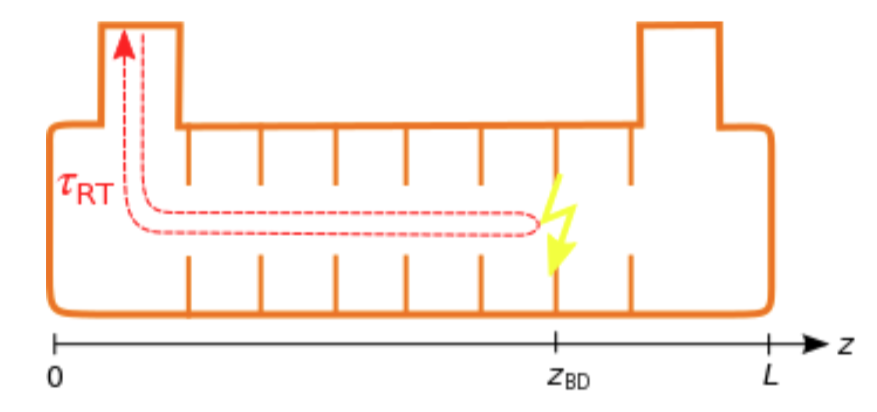
\includegraphics[scale=0.3]{pictures/tToz}
\caption{REF signal path in the accelerating cavity}
\label{tToz_p}
\end{figure}




\section[Final data selection]{Final data selection}
\label{sec:BDR}

The final result of the data selection has to provide the number of breakdowns per run, that will be used to calculate the breakdown rate. 

Ultimately the data selection process that has been described is able to sort out all the fake interlocks and the breakdowns that are happening in the waveguide network or out of the desired experimental conditions. The product of such selection is a group of interesting events that can have taken place in three different regions:
\begin{enumerate}
\item Between the input directional coupler and the input coupling cell (included)
\item In the regular cells of the accelerating structure
\item In the output coupling cell and the waveguide to the RF load
\end{enumerate}
Strictly speaking, only the breakdown happening in the regular cells and in the coupling cells should be counted for the breakdown rate calculation. It is anyway extremely difficult to distinguish between a breakdown happening in the waveguide and in the connected coupling cell. The reason of this is that the group velocity in the regular cell is $\mathcal{O}(\text{0.01 c})$ and in the waveguides is~$\mathcal{O}(\text{c})$. In addition to this, the propagation time of the RF from the directional coupler to the coupling cell is in the order of 4.8 ns (from numerical simulations), which extremely close of the sampling time of 4 ns used in the log detectors. 

In the view of the above considerations, the number of breakdowns and its error are calculated as follows:
\begin{equation}
n_{\text{BD}} \quad \pm \quad \sigma_{\text{Poisson}} \quad \pm \quad \sigma_{\text{Back-off}} 
\label{numBD}
\end{equation}
where  n$_{\text{BD}}$ is the number of breakdowns, $\sigma_{\text{Poisson}}$ is the statistical error on the number of breakdowns and $\sigma_{\text{Back-off}}$ a systematic error coming from the malfunction of the system that misses to back-off immediately the power after a breakdown.

For this kind of experiment, it is acceptable an overestimation of the breakdown rate, but it is not tolerable an underestimation of the breakdown rate. The reason is that an overestimation of the breakdown rate in the tests would lead to a superior performance in CLIC once built, while the opposite is not desirable.   

The components of Eq. \ref{numBD} are calculated according to the following considerations:
\begin{itemize}
\item the number of breakdowns n$_{\text{BD}}$ is the number of breakdowns that are within the metric thresholds.  
\item the poissonian error $\sigma_{\text{Poisson}}$ is used since the breakdown events are rare, it is therefore reasonable think that this phenomenon follows the Poisson's distribution.
\item the missed back-off error contribution $ \sigma_{\text{Back-off}}$ is given from the misbehave of the Xbox. The error is estimated as the number of secondary breakdowns that happens in the next three seconds from an initial one. 
\begin{equation}
\sigma_{\text{Back-off}} = _{- n_{\text{BDs follow-ups}}}^{+ 0}
\end{equation}
\end{itemize}

\noindent
The breakdown rate is finally calculated as
\begin{equation}
BDR = \frac{n_{\text{BD}}}{n_{\text{pulses}}}
\end{equation}
where n$_{\text{pulses}}$ is the number of pulses and is assumed without error. This is a reasonable assumption since the error on the pulse counting is $\pm50$ pulses, while normal measurement runs involve several millions of pulses.